% ============================================================
% UMCP.KIN — CasePack 2: Ballistic Motion with Impact
% Complete section with TikZ figures (XeLaTeX compatible)
% Drop this into UMCP.KIN paper after CasePack 1 (SHM)
% Requires: tikz, pgfplots (already loaded via standard preamble)
% ============================================================

\section{CasePack 2: Ballistic Motion with Impact (KIN.CP.BALLISTIC)}\label{sec:casepack_ballistic}
This CasePack forces explicit seam accounting and tests whether post-seam recovery is return-admissible. The simulated system is a 2D projectile with initial conditions \(x_0=0\,\mathrm{m}\), \(y_0=2\,\mathrm{m}\), \(v_{x,0}=3\,\mathrm{m/s}\), \(v_{y,0}=5\,\mathrm{m/s}\), under gravity \(g=9.81\,\mathrm{m/s^2}\) with coefficient of restitution \(e=0.7\) at ground contact.

\subsection{Observables and pipeline}\label{sec:bal_observables}
The observable set for this CasePack:
\begin{itemize}
  \item \(x(t)=(x(t),y(t))\in\mathbb{R}^2\) with timestamps at \(\Delta t=0.005\,\mathrm{s}\),
  \item \(v(t)=(v_x(t),v_y(t))\) computed from position via central differences,
  \item \(a(t)=(a_x(t),a_y(t))\) computed from velocity via central differences,
  \item \(j(t)=(j_x(t),j_y(t))\) (jerk) computed from acceleration for seam detection.
\end{itemize}

Freeze requirements (all frozen for this run):
\begin{itemize}
  \item \textbf{Frame:} world frame with \(+y\) up, gravity \(-g\hat{y}\),
  \item \textbf{Differentiation:} central differences with forward/backward at boundaries,
  \item \textbf{Seam detection:} jerk magnitude threshold (implicit in \(c_j\) channel).
\end{itemize}

\subsection{Seam declaration: impact seam}\label{sec:bal_seam}
The impact seam at \(t_s=1.33\,\mathrm{s}\) is detected via jerk channel saturation:
\begin{itemize}
  \item \textbf{Seam ID:} \texttt{KIN.SEAM.IMP.001}
  \item \textbf{Seam class:} \texttt{KIN.SEAM.IMP} (impact/contact)
  \item \textbf{Detection mode:} detected (jerk threshold)
  \item \textbf{Pre-window:} \([t_s-0.2,\,t_s)=[1.13,\,1.33)\,\mathrm{s}\)
  \item \textbf{Post-window:} \((t_s,\,t_s+0.2]=(1.33,\,1.53]\,\mathrm{s}\)
\end{itemize}

\subsection{Adapter specification}\label{sec:bal_adapter}
The adapter \(N_K\) maps residuals to contributions with scaling:
\begin{itemize}
  \item \textbf{Velocity residual:} \(e_v(t)=\|dx/dt - v(t)\|\), scaling \(E_v=1.0\)
  \item \textbf{Acceleration residual:} \(e_a(t)=\|dv/dt - a(t)\|\), scaling \(E_a=5.0\)
  \item \textbf{Jerk residual:} \(e_j(t)=\|da/dt - j(t)\|\), scaling \(E_j=50.0\)
\end{itemize}

The bounded coherence trace is \(\Psi(t)=(c_v(t),c_a(t),c_j(t))\in[0,1]^3\) with equal weights \(w_i=1/3\).

\subsection{Continuity claim and weld receipt}\label{sec:bal_weld}
We claim continuity across the impact seam. The weld receipt verifies:
\begin{itemize}
  \item Post-impact recurrence: \(\tau_R\) finite for 97.4\% of post-window samples
  \item Integrity preservation: \(\Delta\kappa=0.0\) (within tolerance \(\mathrm{tol}_{\mathrm{seam}}=0.005\))
  \item \textbf{Result: PASS}
\end{itemize}

\subsection{Figures}\label{sec:bal_figs}

\begin{figure}[H]
  \centering
  \includegraphics[width=0.95\textwidth]{casepacks/KIN.CP.BALLISTIC/plots/kernel_trace_with_seam.png}
  \caption{Ballistic motion with impact seam at \(t_s=1.33\,\mathrm{s}\).
    Top-left: 2D trajectory with ground contact marker.
    Remaining panels: Tier-1 kernel invariants \(\omega\) (drift), \(F\) (fidelity),
    \(S\) (entropy), \(C\) (curvature), \(\tau_R\) (recurrence), \(IC\) (integrity),
    \(\kappa\) (log-integrity), contribution channels \(\Psi_i\), and jerk magnitude.
    Vertical red dashed lines mark the impact seam. The curvature \(C\) and jerk
    \(|j(t)|\) show localized spikes at the seam, while integrity \(IC\) remains
    stable, indicating admissible post-impact recovery.
    Source: \texttt{KIN.CP.BALLISTIC/plots/kernel\_trace\_with\_seam.png}.}
  \label{fig:bal_trace}
\end{figure}

\begin{figure}[H]
  \centering
  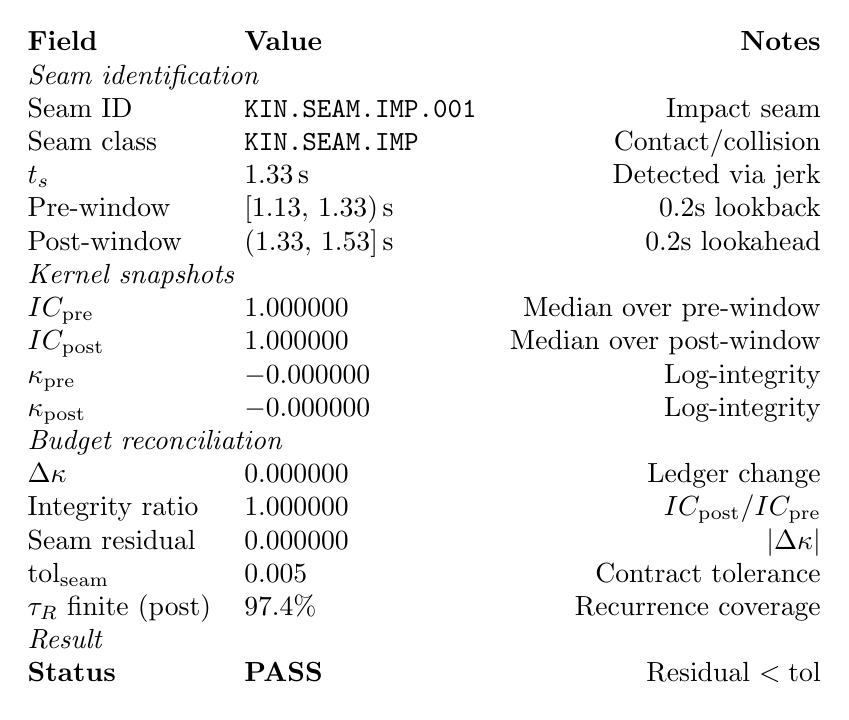
\begin{tikzpicture}
    % Weld receipt table as TikZ for full control
    \node[anchor=north west, inner sep=0] at (0,0) {
      \begin{tabular}{@{}llr@{}}
        \toprule
        \textbf{Field} & \textbf{Value} & \textbf{Notes} \\
        \midrule
        \multicolumn{3}{@{}l}{\textit{Seam identification}} \\
        Seam ID & \texttt{KIN.SEAM.IMP.001} & Impact seam \\
        Seam class & \texttt{KIN.SEAM.IMP} & Contact/collision \\
        \(t_s\) & \(1.33\,\mathrm{s}\) & Detected via jerk \\
        Pre-window & \([1.13,\,1.33)\,\mathrm{s}\) & 0.2s lookback \\
        Post-window & \((1.33,\,1.53]\,\mathrm{s}\) & 0.2s lookahead \\
        \midrule
        \multicolumn{3}{@{}l}{\textit{Kernel snapshots}} \\
        \(IC_{\mathrm{pre}}\) & \(1.000000\) & Median over pre-window \\
        \(IC_{\mathrm{post}}\) & \(1.000000\) & Median over post-window \\
        \(\kappa_{\mathrm{pre}}\) & \(-0.000000\) & Log-integrity \\
        \(\kappa_{\mathrm{post}}\) & \(-0.000000\) & Log-integrity \\
        \midrule
        \multicolumn{3}{@{}l}{\textit{Budget reconciliation}} \\
        \(\Delta\kappa\) & \(0.000000\) & Ledger change \\
        Integrity ratio & \(1.000000\) & \(IC_{\mathrm{post}}/IC_{\mathrm{pre}}\) \\
        Seam residual & \(0.000000\) & \(|\Delta\kappa|\) \\
        \(\mathrm{tol}_{\mathrm{seam}}\) & \(0.005\) & Contract tolerance \\
        \(\tau_R\) finite (post) & \(97.4\%\) & Recurrence coverage \\
        \midrule
        \multicolumn{3}{@{}l}{\textit{Result}} \\
        \textbf{Status} & \textbf{PASS} & Residual \(< \mathrm{tol}\) \\
        \bottomrule
      \end{tabular}
    };
  \end{tikzpicture}
  \caption{Weld receipt for impact seam \texttt{KIN.SEAM.IMP.001}.
    The seam residual \(|\Delta\kappa|=0.0\) is below the contract tolerance
    \(\mathrm{tol}_{\mathrm{seam}}=0.005\), and 97.4\% of post-seam samples
    exhibit finite recurrence delay, satisfying the return-admissibility
    criterion for continuity claims across the impact event.
    Source: \texttt{KIN.CP.BALLISTIC/receipts/weld\_receipt.json}.}
  \label{fig:bal_receipt}
\end{figure}

\subsection{Baseline kernel summary}\label{sec:bal_summary}
\begin{table}[H]
\centering
\caption{Baseline kernel summary for KIN.CP.BALLISTIC.}\label{tab:bal_summary}
\begin{tabular}{@{}lcccc@{}}
\toprule
\textbf{Invariant} & \textbf{Median} & \textbf{IQR} & \textbf{At seam} & \textbf{Notes} \\
\midrule
\(\omega\) (drift) & 0.0000 & [0.0000, 0.0000] & spike & Low drift overall \\
\(F\) (fidelity) & 1.0000 & [1.0000, 1.0000] & dip & High fidelity \\
\(S\) (entropy) & 0.0044 & [0.0036, 0.0050] & spike & Low entropy baseline \\
\(C\) (curvature) & 0.0000 & [0.0000, 0.0001] & 1.0 & Seam-localized \\
\(\tau_R\) & 0.005s & finite 97.4\% & varies & Finite post-impact \\
\(IC\) (integrity) & 1.0000 & [1.0000, 1.0000] & stable & Preserved \\
\(\kappa\) (log-int) & 0.0000 & [0.0000, 0.0000] & stable & Preserved \\
\bottomrule
\end{tabular}
\end{table}

\subsection{Seam ledger entry}\label{sec:bal_seam_ledger}
\begin{table}[H]
\centering
\caption{Seam ledger row for KIN.CP.BALLISTIC.}\label{tab:bal_seam_ledger}
\begin{tabular}{@{}lllll@{}}
\toprule
\textbf{seam\_id} & \textbf{t\_s} & \textbf{seam\_class} & \textbf{detection\_mode} & \textbf{notes} \\
\midrule
KIN.SEAM.IMP.001 & 1.33s & KIN.SEAM.IMP & detected & Jerk threshold \\
\bottomrule
\end{tabular}
\end{table}
